https://atcoder.jp/contests/abc285/editorial/5535

On the resulting graph, 
accumulate maximum flow in the following order:
* from S' to T'
* from S' to T
* from S to T'
* from S to T.

An S-T flow that satisfies the minimum capacities 
exists if and only if, for all outgoing edges 
from S' and incoming edges to T', 
the flow and capacity are equal.

\begin{center}\begin{minipage}{50mm}
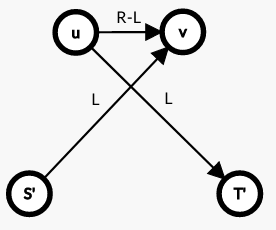
\includegraphics[width=\textwidth]{content/graphs/max-flow-min-capacities.png}
\end{minipage}\end{center}
